\newcommand{\nterm}[1]{#1}
\newcommand{\term}[1]{#1}
\newcommand{\filename}[1]{\mbox{\texttt{#1}}}

\chap{系统测试}

BO 编译器的目的是将使用 BO 语言编写的源程序转化为等价的 BOVM 虚拟机能够理解的目标语言程序。如果 BO 编译器存在面对特定输入崩溃、目标代码的行为与源程序语义不一致、错误提示信息有误等问题,可能导致使用 BO 语言的开发人员找不到错误根源,或者用 BO 语言编写的应用程序存在严重问题。因此编译器的可靠性十分关键,我们有必要通过系统化测试找出编译器存在的潜在问题、检验编译器的质量\cite{emark2012}。

\sect{程序运行过程测试}
如图 \ref{fig_test_hello} 所示,\filename{hello.bo} 文件中仅含一条 \verb|println('Hello world!')| 语句。使用 boc 命令产生 \filename{hello.boc} 文件,随后使用 bo 命令执行。BO编译器与BOVM虚拟机运行正常,结果输出 \verb|Hello world!| ,符合预期。
\begin{figure}[H]
    \centering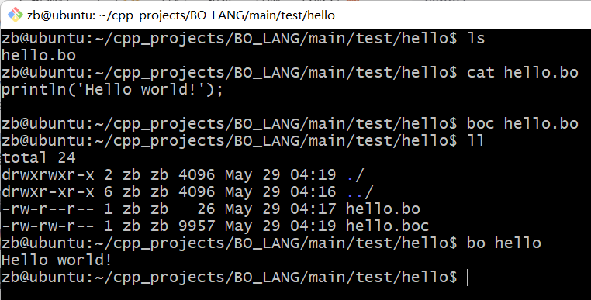
\includegraphics[]{figure/test_hello.pdf}
    \caption{\filename{hello.bo} 文件的编译与运行}
    \label{fig_test_hello}
\end{figure}

\sect{语句测试}

(1) 表达式语句测试

表达式语句的测试用例及运行结果如图 \ref{fig_test_expression} 所示。文件 \filename{expression\_test.bo} 通过直接输出各种表达式的结果进行测试。可见,常量表达式、算术表达式、布尔表达式、以及赋值表达式的结果均符合预期。

\begin{figure}[H]
    \centering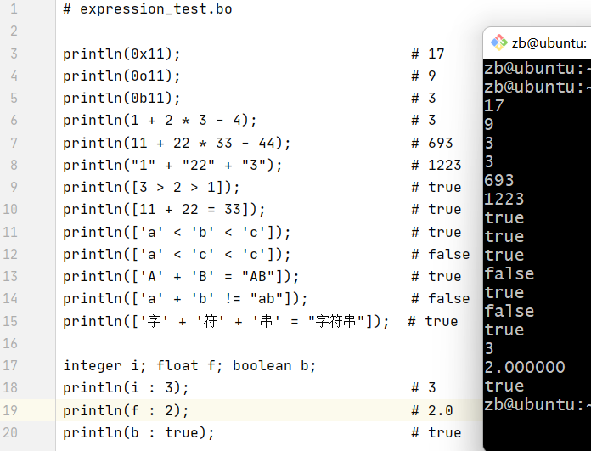
\includegraphics{figure/test_expression.pdf}
    \caption{表达式语句测试}
    \label{fig_test_expression}
\end{figure}


(2) if 语句测试

if 语句的测试用例及运行结果如图 \ref{fig_test_if} 所示。 \verb|if_test| 函数根据形参 a 的值判断它所属的区间,19 到 22 行循环调用函数进行判断,结果符合预期。

\begin{figure}[H]
    \centering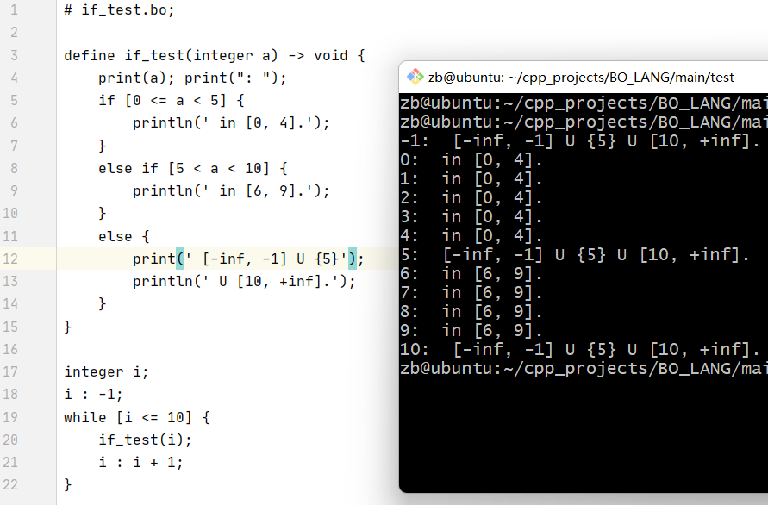
\includegraphics{figure/test_if.pdf}
    \caption{if 语句测试}
    \label{fig_test_if}
\end{figure}

(3) switch 语句测试

switch 语句的测试用例及运行结果如图 \ref{fig_test_switch} 所示。 \verb|switch_test| 函数中的switch语句根据形参 a 的值执行不同的代码块,结果符合预期。

\begin{figure}[H]
    \centering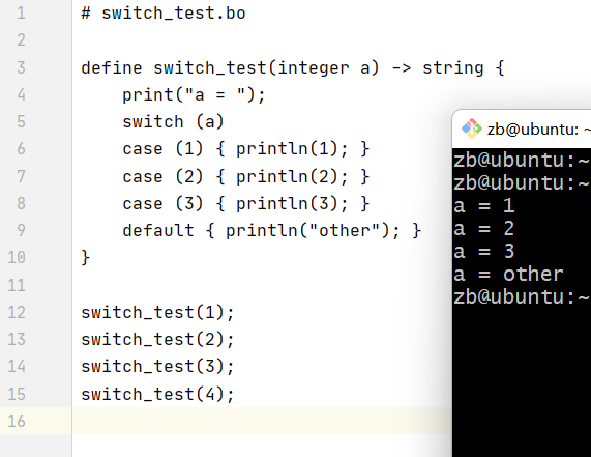
\includegraphics{figure/test_switch.pdf}
    \caption{switch 语句测试}
    \label{fig_test_switch}
\end{figure}

(4) while 语句测试

while 语句的测试用例及运行结果如图 \ref{fig_test_while} 所示。 \verb|isPrime| 函数判断形参 num 是否为素数,第 16 行的 while 语句循环打印数字1到99中的素数,结果符合预期。

\begin{figure}[H]
    \centering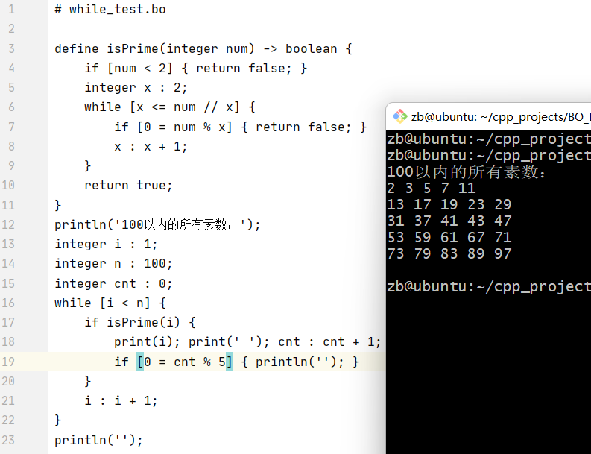
\includegraphics{figure/test_while.pdf}
    \caption{while 语句测试}
    \label{fig_test_while}
\end{figure}

(5) repeat 语句测试

repeat 语句的测试用例及运行结果如图 \ref{fig_test_repeat} 所示。第 8 行的 repeat 语句会执行 end$-$start 次,结果符合预期。

\begin{figure}[H]
    \centering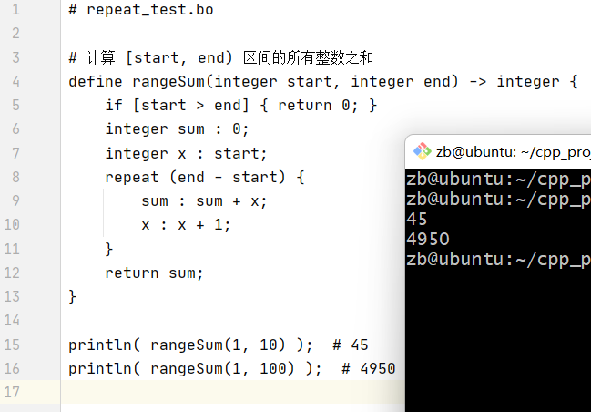
\includegraphics{figure/test_repeat.pdf}
    \caption{repeat 语句测试}
    \label{fig_test_repeat}
\end{figure}

\sect{函数与类的测试}

(1)函数递归测试

函数递归的测试用例及运行结果如图 \ref{fig_test_recur} 所示。 \verb!factorial! 函数递归计算 $n!$ ,结果符合预期。

\begin{figure}[H]
    \centering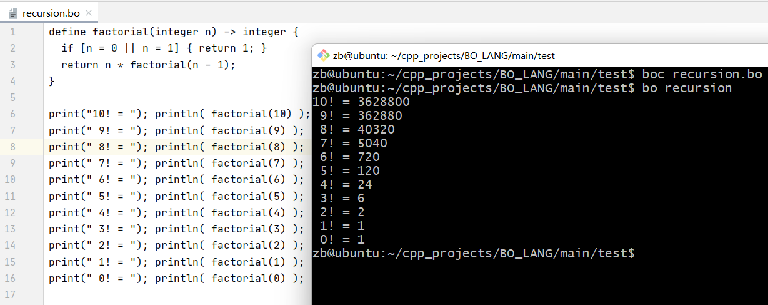
\includegraphics{figure/test_recursion.pdf} 。
    \caption{factorial 函数递归测试}
    \label{fig_test_recur}
\end{figure}

(2)类测试

类测试用例及运行结果如图 \ref{fig_test_class} 所示。 Animal 类被声明为 abstract,代表可被继承,它有一个 type 属性和两个可被覆盖(声明为virtual)的方法,其中 type 代表动物名称、constructor是声明构造方法的关键字; Dog 和 Cat 分别继承了 Animal 类并重写了两个方法。第 19 和 20 行通过父类指针实现多态,运行结果符合预期。

\begin{figure}[H]
    \centering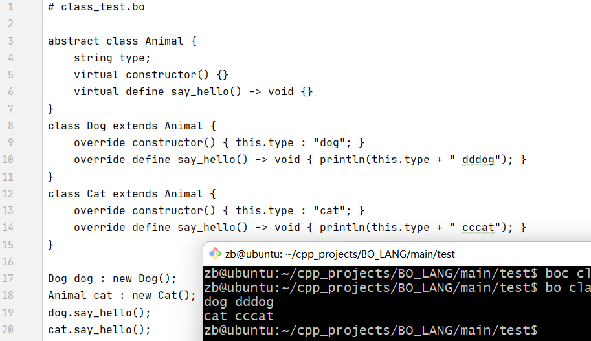
\includegraphics{figure/test_class.pdf}
    \caption{类测试}
    \label{fig_test_class}
\end{figure}

\sect{变量作用域测试}

变量作用域测试用例及运行结果如图 \ref{fig_test_scope} 所示, \filename{test\_scope.bo} 文件中,顶层结构、 if 语句和 func 函数体内各有一个变量 a 的定义。
% 第 2 行变量 a 的作用域是 fun 函数体内,第 7 行变量 a 的作用域是顶层结构,第 11 行的变量 a 的作用域是 if 语句的代码块。
它们的作用域是它们所在的代码块中自身定义位置之后的范围。因此第 10 行的变量 a 定义在第 7 行。测试结果符合预期。
\begin{figure}[H]
    \centering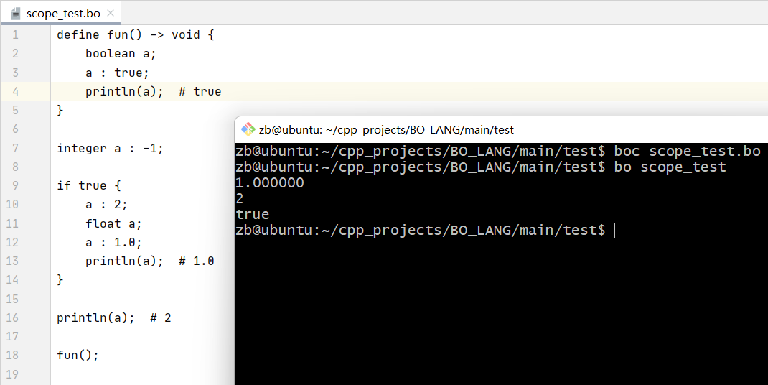
\includegraphics{figure/test_scope.pdf}
    \caption{变量作用域测试}
    \label{fig_test_scope}
\end{figure}

\sect{代码优化测试}

代码优化效果无法直接从 BO 编译器的运行结果观察,因此我们采用 bop 命令可视化查看编译生成的 \filename{.boc} 文件中的字节码。真正的字节码仅由二进制的 0 和 1 组成, bop 命令会将其解析为助忆符的形式展现。

(1)表达式语句代码优化测试

表达式语句代码优化测试用例及运行结果如图 \ref{test_optimizer1} 所示。表达式 $1+2*3-\text{t}$ 折叠成为 $7-\text{t}$ ,表达式 $\text{t}+2*3-4$ 折叠成为 $\text{t}+6-4$ 。测试结果符合预期。

\begin{figure}[H]
\centering
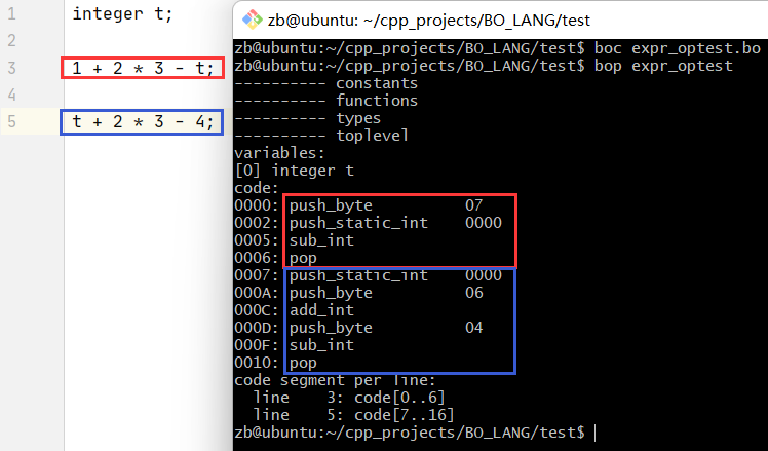
\includegraphics{figure/test_optimizer1.pdf}
\caption{表达式语句代码优化测试}
\label{test_optimizer1}
\end{figure}

(2)if 语句代码优化测试

if 语句代码优化测试用例及运行结果如图 \ref{test_optimizer2} 所示。条件为true的if块被展开,条件为false的if块被消去。测试结果符合预期。

\begin{figure}[H]
\centering
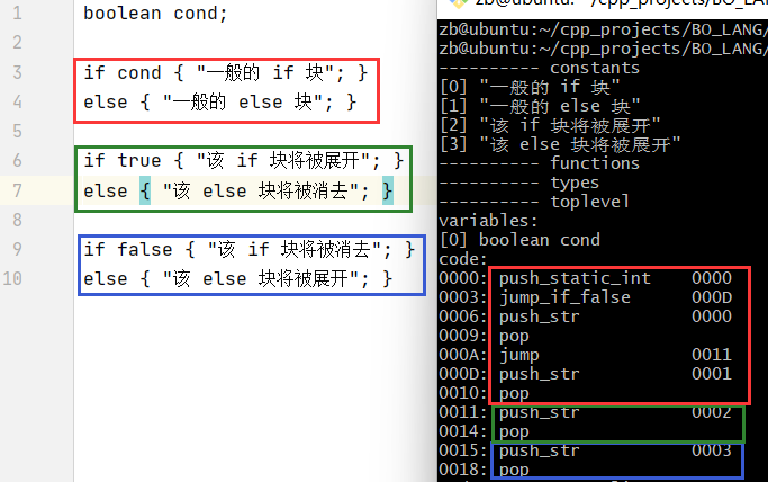
\includegraphics{figure/test_optimizer2.pdf}
\caption{if 语句代码优化测试}
\label{test_optimizer2}
\end{figure}

(2)while 语句代码优化测试

while 语句代码优化测试用例及运行结果如图 \ref{test_optimizer3} 所示。break语句之后的字节码被消去。测试结果符合预期。

\begin{figure}[H]
\centering
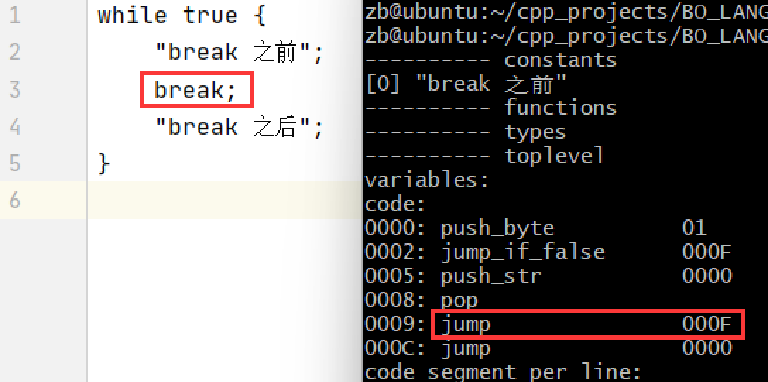
\includegraphics{figure/test_optimizer3.pdf}
\caption{while 语句代码优化测试}
\label{test_optimizer3}
\end{figure}

(2)repeat 语句代码优化测试

repeat 语句代码优化测试用例及运行结果如图 \ref{test_optimizer4} 所示。循环 0 次的代码块直接消去,循环 1 次的代码块直接展开。测试结果符合预期。

\begin{figure}[H]
\centering
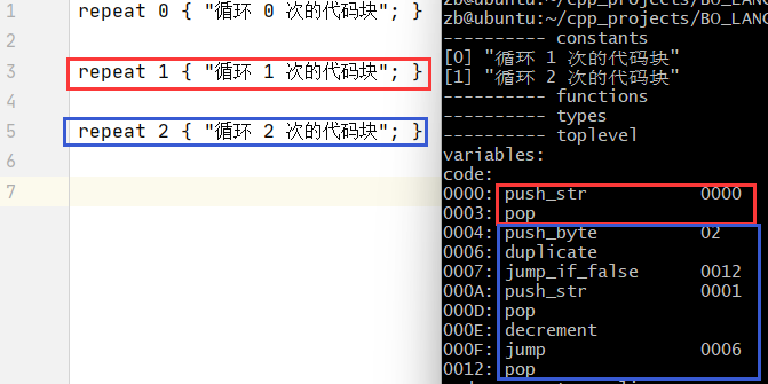
\includegraphics{figure/test_optimizer4.pdf}
\caption{repeat 语句代码优化测试}
\label{test_optimizer4}
\end{figure}

\sect{错误处理测试}

 BO 编译器一旦发现语法或语义错误便会立即报告当前错误并终止,因此我们只需构造存在一条错误语句的程序进行测试即可。

(1)词法错误处理测试

词法错误处理测试用例及运行结果如图 \ref{fig_test_scanner_error} 所示,编译器指出在 \filename{scanner\_error\_test.bo} 文件的第 10 行 7 列在非注释环境下出现了一个非法字符 \verb!@! 。由于此时尚未进行语义分析,所以编译器尚未发现第 3 行存在未定义标识符,运行结果符合预期。

\begin{figure}[H]
    \centering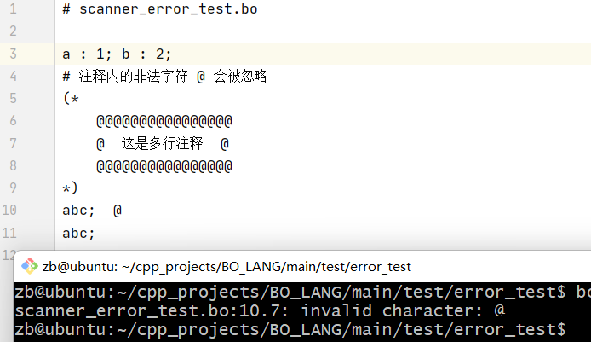
\includegraphics[width=13cm]{figure/test_scanner_error.pdf}
    \caption{词法错误处理测试}
    \label{fig_test_scanner_error}
\end{figure}

(2)语法错误处理测试

语法错误处理测试用例及运行结果如图 \ref{fig_test_parser_error} 所示,编译器指出在第 5 行 1 列识别到了一个非预期的标识符,并表示预期读入一个分号。由于此时尚未进行语义分析,所以编译器尚未发现第 3 行存在未定义标识符,运行结果符合预期。

\begin{figure}[H]
    \centering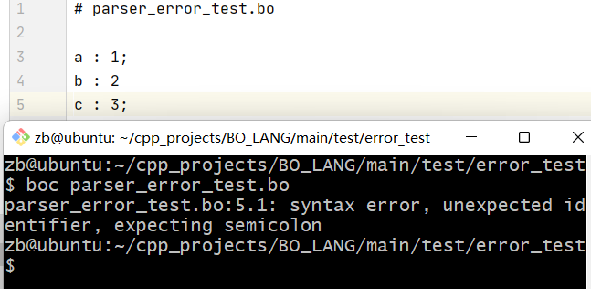
\includegraphics[width=13cm]{figure/test_parser_error.pdf}
    \caption{语法错误处理测试}
    \label{fig_test_parser_error}
\end{figure}

(3)语义错误处理测试

语义错误处理测试用例及运行结果如图 \ref{fig_test_semantic_error} 所示,编译器指出在第 10 行类成员 b 不可访问,结果符合预期。

\begin{figure}[H]
    \centering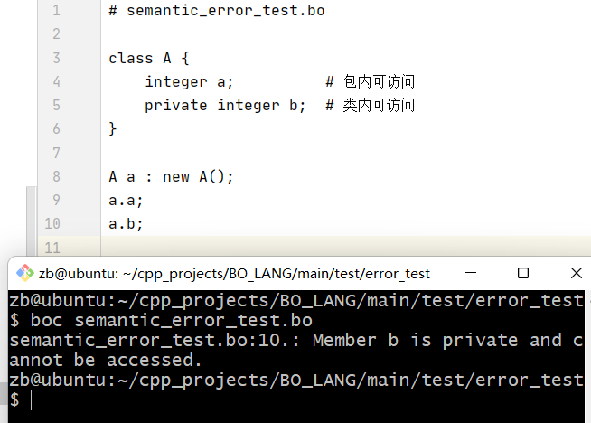
\includegraphics[width=13cm]{figure/test_semantic_error.pdf}
    \caption{语义错误处理测试}
    \label{fig_test_semantic_error}
\end{figure}


% \sect{性能测试}







\let\nterm\undefined
\let\term\undefined
\let\filename\undefined







% 假设已存在定义 \verb!integer i;! \verb!float f;! \verb!boolean b;! \verb!string s;! 。对表达式语句的测试如表 \ref{tab_test_expr} 所示。
% \newcommand{\widthOfRes}{4cm}
% \begin{table}[H]
% \centering
% \caption{表达式语句测试用例}
% \begin{tabular}[]{@{}lllll@{}}
%     \toprule
%     类型         & 表达式                         & 预期结果      & 实际结果   &  是否通过                       \\
%     \midrule
%     十六进制整型    &  \verb!0x11!                &  17           & 17                           &   通过                    \\
%     八进制整型      &  \verb!0o11!                &  9            & 9                            &   通过                    \\
%     二进制整型      &  \verb!0b11!                &  3            & 3                            &   通过                    \\
%     算术表达式      &  \verb!11 + 22 * 33 - 44!   &  693          & 693                          &   通过                    \\
%     布尔表达式      &  \verb![3 > 2 > 1]!         &  true         & true                         &   通过                    \\
%     布尔表达式      &  \verb!['a' < 'b' < 'c']!   &  true         & true                         &   通过                    \\
%     布尔表达式      &  \verb!['a' < 'd' < 'c']!   &  false        & false                        &   通过                    \\
%     布尔表达式      &  \verb!['A' + 'B' = "AB"]!  &  true         & true                         &   通过                    \\
%     非法表达式      &  \verb!i = 1!               & 语法错误       & \parbox[t]{\widthOfRes}{unexpected token: =}  &   通过                    \\
%     赋值表达式      &  \verb!i : 1!               & 1             & 1  &   通过                    \\ 
%     赋值表达式      &  \verb!i : s!               & 语义错误       & \parbox[t]{\widthOfRes}{Cannot cast from string to integer.}  &   通过                    \\ 
%     赋值表达式      &  \verb!f : 2!               & 2.000000       & 2.000000  &   通过                    \\ 
%     加法表达式      &  \verb!i + b!               & 语义错误       & \parbox[t]{\widthOfRes}{The operand type of the arithmetic operator is invalid.}  &   通过                    \\ 
%     非法表达式      &  \verb!@abc!               & 词法错误       & \parbox[t]{\widthOfRes}{invalid character: @}  &   通过                    \\
%     \bottomrule
% \end{tabular}
% \label{tab_test_expr}
% \end{table}
% \let\widthOfRes\undefined


%%%%%%%%%%%%%%%%%%%%%%%%%%%%%%%%%%%%%%%%%%%%%%%%%%%%%%%%%%%%%%%%%%%%%%%
%%%%%%%%%%%%%%%%%%%%%%%%%%%%%%%%%%%%%%%%%%%%%%%%%%%%%%%%%%%%%%%%%%%%%%%
%%%%%%%%%%%%%%%%%%%%%%%%%%%%%%%%%%%%%%%%%%%%%%%%%%%%%%%%%%%%%%%%%%%%%%%
%%%%%%%%%%%%%%%%%%%%%%%%%%%%%%%%%%%%%%%%%%%%%%%%%%%%%%%%%%%%%%%%%%%%%%%
%%%%%%%%%%%%%%%%%%%%%%%%%%%%%%%%%%%%%%%%%%%%%%%%%%%%%%%%%%%%%%%%%%%%%%%
%%%%%%%%%%%%%%%%%%%%%%%%%%%%%%%%%%%%%%%%%%%%%%%%%%%%%%%%%%%%%%%%%%%%%%%


% 假设已存在如图 \ref{fig_class_def} 所示类 Animal、Dog、Cat、Person 以及相关变量的定义。对类的封装、继承和多态的测试如表 \ref{tab_test_class} 所示。
% 
% \begin{figure}[H]
% \centering
% \begin{subfigure}[b]{.45\textwidth}
% \vspace{0pt}
% \centering
% \begin{lstlisting}[numbers=none]
% abstract class Animal {
%     virtual define sayHello() -> void {}
% }
% class Dog extends Animal {
%     override sayHello() -> void {
%         println("dog hello");
%     }
% }
% class Cat extends Animal {
%     override sayHello() -> void {
%         println("cat hello");
%     }
% }
% \end{lstlisting}
% \caption{类 Animal 及其子类的定义}
% % \label{fig_func_call_expr_2}
% \end{subfigure}
% \quad\quad
% \begin{subfigure}[b]{.45\textwidth}
% \vspace{0pt}
% \centering
% \begin{lstlisting}[numbers=none]
% class Person {
%     public string name;
%     private integer age;
%     define constructor
%     initialize(string name, integer age) {
%         this.name : name;
%         this.age : age;
%     }
% }
% Person p1 : new Person("Bob", 22);
% Person p2;
% Animal dog : new Dog();
% Animal cat : new Cat();
% \end{lstlisting}
% \caption{类 Object 与变量的定义}
% % \label{fig_func_call_expr_2}
% \end{subfigure}
% \caption{待测试类的定义}
% \label{fig_class_def}
% \end{figure}

% \newcommand{\widthOfRes}{4cm}
% \begin{table}[H]
% \centering
% \caption{流程控制语句测试用例}
% \begin{tabular}[]{@{}lllll@{}}
%     \toprule
%     类型           & 表达式           & 预期结果      & 实际结果   &  是否通过                       \\
%     \midrule
%     类成员访问表达式  &  p1.name         &  Bob           & Bob                          &   通过                    \\
%     类成员访问表达式  &  p1.age          &  语法错误       & Member age is private.       &   通过                    \\
%     类成员访问表达式  &  p2.name         &  空指针异常     & Exception occured: null pointer.     &   通过                    \\
%     类成员访问表达式  &  dog.sayHello()  &  dog hello     & dog hello                          &   通过                    \\
%     类成员访问表达式  &  cat.sayHello()  &  cat hello     & cat hello                         &   通过                    \\
%     \bottomrule
% \end{tabular}
% \label{tab_test_class}
% \end{table}
% \let\widthOfRes\undefined

% \FloatBarrier

% \FloatBarrier


% \sect{功能测试}
% \subsec{表达式语句测试}

% \subsec{流程控制语句测试}
% 假设已存在如图 \ref{fig_func_def} 所示 getGrade 与 rangeSum 的函数定义。对流程控制语句的测试如表 \ref{tab_test_con} 所示。


% \begin{figure}[H]
% \centering
% \begin{subfigure}[b]{.45\textwidth}
% \vspace{0pt}
% \centering
% \begin{lstlisting}[numbers=none]
% # 根据分数判断等级
% define getGrade(integer score) -> string {
%     string grade : null;
%     if [score >= 90] { grade : 'A'; }
%     else if [score >= 80] { grade : 'B'; }
%     else if [score >= 60] { grade : 'C'; }
%     else { grade : 'D'; }
%     return grade;
% }
% \end{lstlisting}
% \caption{getGrade 函数定义}
% % \label{fig_func_call_expr_2}
% \end{subfigure}
% \quad
% \begin{subfigure}[b]{.5\textwidth}
% \vspace{0pt}
% \centering
% \begin{lstlisting}[numbers=none]
% # 计算 [start, end) 区间的所有整数之和
% define rangeSum(integer start, integer end) 
%     -> integer {
%     if [start > end] { return 0; }
%     integer sum : 0;
%     integer x : start;
%     while [x != end] {
%         sum : sum + x;
%         x : x + 1;
%     }
%     return sum;
% }
% \end{lstlisting}
% \caption{rangeSum 函数定义}
% % \label{fig_func_call_expr_2}
% \end{subfigure}
% \caption{待测试函数定义}
% \label{fig_func_def}
% \end{figure}

% \newcommand{\widthOfRes}{4cm}
% \begin{table}[H]
% \centering
% \caption{流程控制语句测试用例}
% \begin{tabular}[]{@{}lllll@{}}
%     \toprule
%     类型         & 表达式或语句                         & 预期结果      & 实际结果   &  是否通过                       \\
%     \midrule
%     函数调用表达式  &  getGrade(95)  &  A           & A                           &   通过                    \\
%     函数调用表达式  &  getGrade(85)  &  B            & B                            &   通过                    \\
%     函数调用表达式  &  getGrade(75)  &  C            & C                            &   通过                    \\
%     函数调用表达式  &  getGrade(60)  &  C          & C                          &   通过                    \\
%     函数调用表达式  &  getGrade(59)  &  D         & D                         &   通过                    \\
%     函数调用表达式  &  getGrade(45)  &  D         & D                         &   通过                    \\
%     函数调用表达式  &  rangeSum(1, 10)  &  45         & 45                         &   通过                    \\
%     函数调用表达式  &  rangeSum(1, 100)  &  4950         & 4950                         &   通过                    \\
%     非法 if 语句        &  if (true) ;   & 语法错误    & unexpected ;, expecting \verb!{!   & 通过  \\
%     if 语句        &  if (true) {}   & 正常运行    & 正常运行   & 通过  \\
%     非法 if 语句        &  if (1) {}   & 语义错误    & \parbox[t]{\widthOfRes}{The conditional expression must be a boolean type.}   & 通过  \\
%     \bottomrule
% \end{tabular}
% \label{tab_test_con}
% \end{table}
% \let\widthOfRes\undefined
